% =========================================================================== %
% TeX input file: "download and install scout"
%
% WARNING: this tex file does not compile standalone, it needs to be embedded
% in a master tex document (e.g. ScoutInstallation.tex)
% =========================================================================== %

Before you download Scout make sure that you have a working Java Development Kit (JDK) of version 7 or 8.
To download Eclipse Scout visit the official Eclipse download page.

\url{https://www.eclipse.org/downloads/}

The download page then looks as shown in \figref{scout_download}.
If the download page shows the wrong platform, manually select the correct platform in the dropdown list.

\begin{figure}
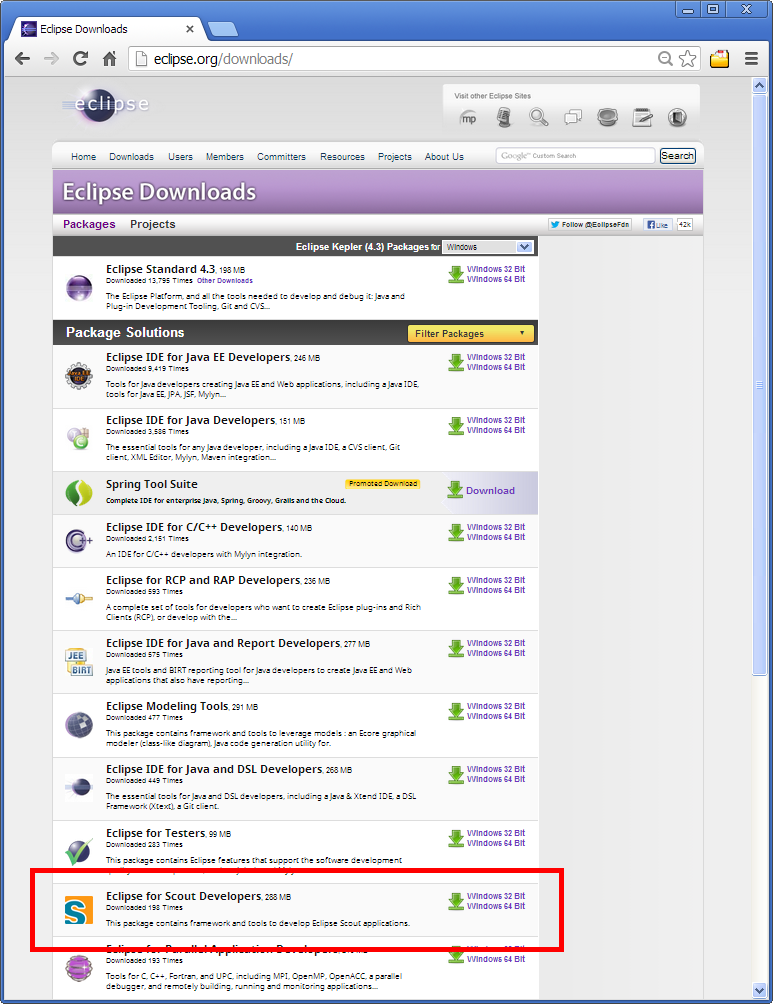
\includegraphics[width=15cm]{scout_download.png}
\caption{The Eclipse download page. The platform filter is set to Windows and the available Packages are filtered for Scout.}
\figlabel{scout_download}
\end{figure}

The Eclipse Scout package is available in the form of a 32 bit and a 64 bit package as shown in\figref{scout_download}. 
To download the correct package, make sure to matche your JDK installation. 
You can check your installation on the command line as follows.

\begin{lstlisting}[
  language=console
]
console-prompt>java -version
java version "1.7.0_55"
Java(TM) SE Runtime Environment (build 1.7.0_55-b13)
Java HotSpot(TM) 64-Bit Server VM (build 24.55-b03, mixed mode)
\end{lstlisting}

If the output explicitly mentions the 64 bit installation as shown in the example above, you have a 64 bit installation and you need to download the 64 bit Eclipse Scout package. 
Otherwise, you have a 32 bit JDK installed and you need to pick the 32 bit package of Eclipse Scout.
After the package selection, confirm the suggested download mirror as shown in \figref{scout_download_mirror}.

\begin{figure}
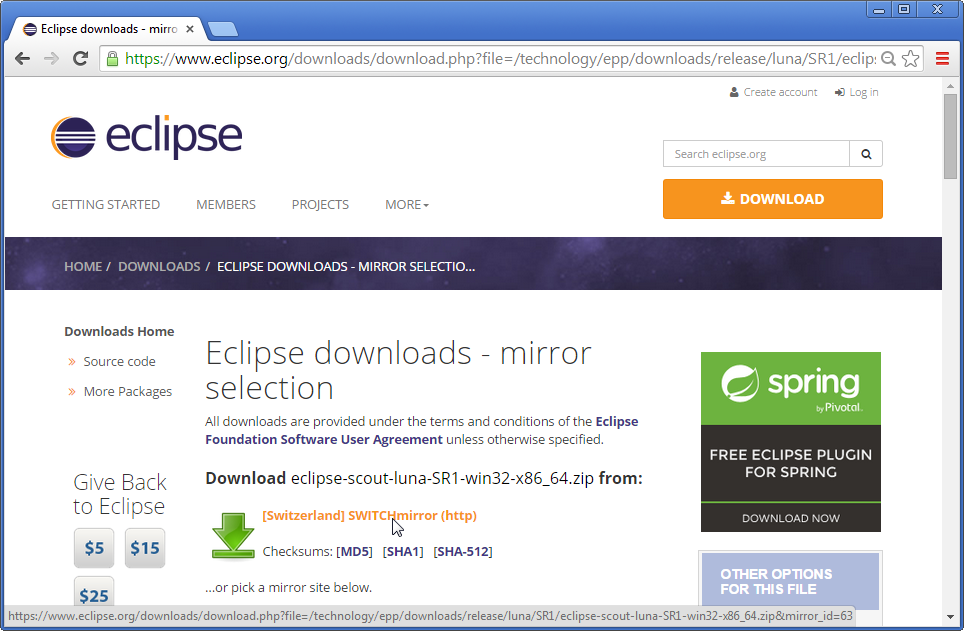
\includegraphics[width=15cm]{scout_download_mirror.png}
\caption{Downloading the Scout package from a mirror.}
\figlabel{scout_download_mirror}
\end{figure}

% =========================================================================== %
% EOF TeX input file
% =========================================================================== %
